\documentclass{article}
\usepackage[utf8]{inputenc}
\usepackage[dutch]{varioref}
\usepackage[autostyle]{csquotes} 
\usepackage[dutch]{babel}
\usepackage{listings}
\usepackage{pdfpages}
\usepackage{url}
\usepackage{natbib}
\usepackage{graphicx}

\lstset{
    frame=single,
    breaklines=true,
    postbreak=\raisebox{0ex}[0ex][0ex]{\ensuremath{\color{red}\hookrightarrow\space}}
}

\title{Stageverslag}
\author{\mbox{Pieter-Jan} Robrecht}
\date{Maart 2016}

\begin{document}

%\maketitle
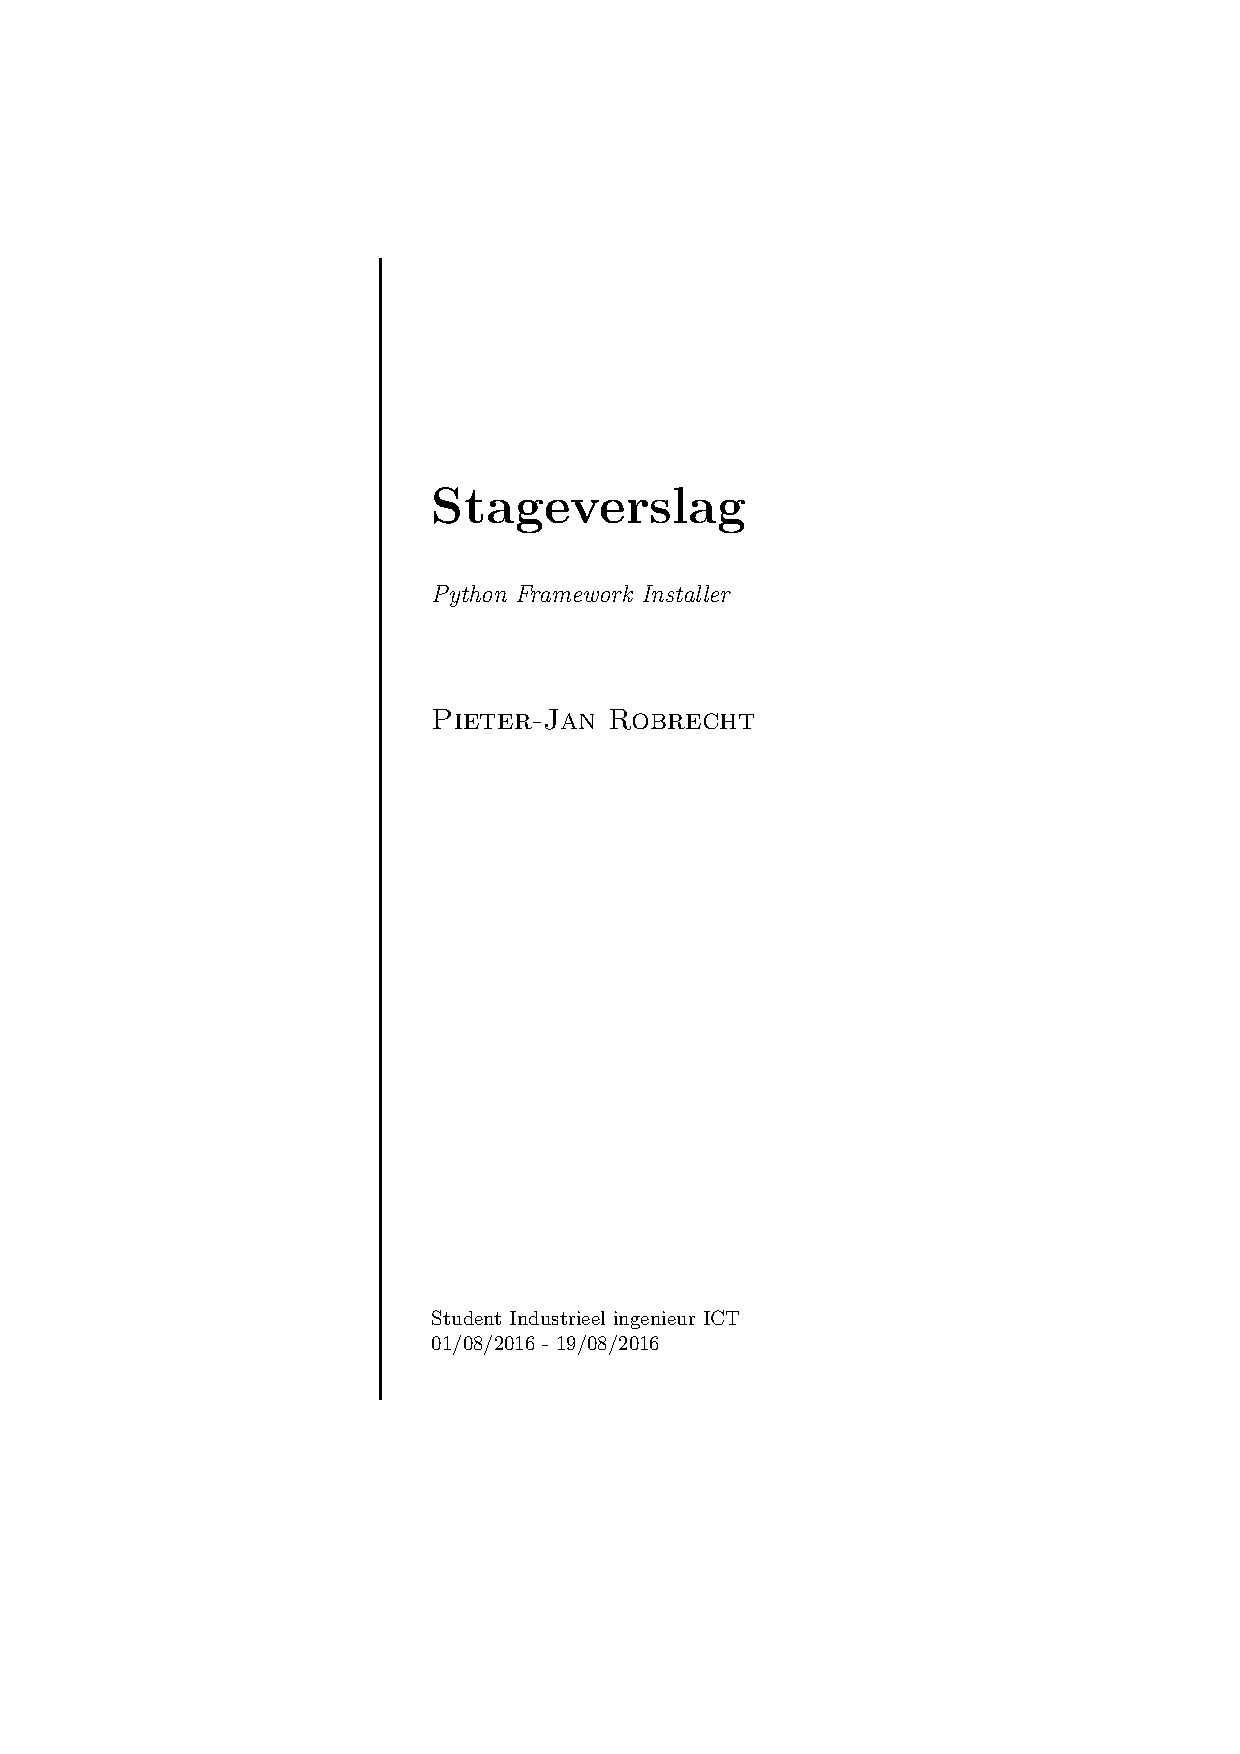
\includepdf{titel/titelstage.pdf}

%Volgende lijn is om de titelpagina geen paginanummer te geven
\clearpage
\setcounter{page}{1}

\tableofcontents
\lstlistoflistings
\clearpage

\section{Inleiding}
In het kader van mijn masterproef was het mogelijk om bij Televic Rail een stage te lopen tijdens de zomer. 
Gedurende deze stage heb ik mijn masterproef voorbereid en onderzoek gedaan naar de verschillende mogelijkheden die er zijn voor het uitvoeren van mijn opdracht.
De opdracht die voltooid moet worden is de volgende:

\begin{displayquote}
Televic Rail heeft een Python test framework ontworpen. 
Dit framework werd oorspronkelijk gebruikt op een volledig uitgeruste testtoren, maar het framework werd aangepast zodanig dat het onafhankelijk van de testtoren gebruikt kan worden.
Aangezien het framework gebruik maakt van verschillende niet-standaard Python bibliotheken, is het installeren van het framework op een nieuw systeem een hele klus.
Het doel is dan ook het maken van een installer-updater waarmee dit proces kan worden vergemakkelijkt zodanig dat er zo min mogelijk interactie van de gebruiker moet zijn.
\end{displayquote}

Tijdens de duur van de stage werden er verschillende implementatie manieren onderzocht en werd er een algemene architectuur voor de installer-updater uitgedacht.
In wat volgt wordt er beschreven welke stappen er werden overlopen om het probleem onder te verdelen in enkele logische onderdelen en we zoeken naar een oplossing om deze op te lossen. 

\section{Analyse van het probleem}\label{section:analyse}
Tijdens het bespreken van het probleem werd het al snel duidelijk dat er verschillende scenario's zijn waarin het framework gebruikt wordt. 
Het framework wordt als een standalone programma gebruikt op een laptop of desktop maar het zal ook moeten draaien op verschillende testtorens. 
Voor de verschillende omgevingen zal iedere keer een andere configuratie nodig zijn maar beiden omgevingen gebruiken Windows als besturingssysteem.
Uiteraard moeten we ervan uitgaan dat deze situatie slechts tijdelijk is.
Er wordt best een applicatie geschreven die op meer dan enkel Windows kan draaien.

Tijdens het installeren van het framework moeten we rekening houden met het feit dat iedere computer een andere configuratie en andere drivers zal nodig hebben.
We kunnen de gebruiker vragen om de verschillende drivers te selecteren, maar, mocht het mogelijk zijn, dan zou de applicatie best zelf de verschillende devices detecteren om vervolgens zelf de juiste drivers aan te vinken in de volledige lijst van drivers.
Zo moet de gebruiker minder weet hebben van welke drivers er allemaal nodig zijn.
Het probleem van de drivers beperkt zich jammer genoeg niet enkel tot dit.
Als er nieuwe hardware ontwikkelt wordt, zullen er ook verschillende nieuwe drivers nodig zijn.
De lijst van beschikbare drivers zal dan tijdig moeten worden aangepast.
Er zal dus ergens een volledige lijst moeten zijn met alle devices en welke drivers eraan gekoppeld zijn.
Deze lijst zou dan eventueel ook de laatste versienummers hebben.
De updater kan deze lijst dan ook gebruiken om te controleren of de versie van de ge\"installeerde drivers de laatste versie is.

De installer is best ook een programma dat zo eenvoudig mogelijk uit te breiden of aan te passen is zodanig dat het in de toekomst nog kan worden aangepast. 
De interface naar de gebruiker toe is best ook zo eenvoudig mogelijk zodanig dat er geen problemen kunnen ontstaan tijdens de installatie/update van het framework.
Uiteraard gaan we er vanuit moeten gaan dat er af en toe een probleem zal ontstaan tijdens de installatie.
De installatie/updates zullen dus best in een afgesloten omgeving uitgevoerd worden en na het correct uitvoeren in het grote geheel geplaatst worden.

De updater bezit gelijkaardige problemen.
We zullen een manier moeten vinden waarmee we gemakkelijk kunnen controleren naar de versienummers van de software.
De gebruiker zal ook de optie moeten krijgen om de update uit te voeren.
De gebruiker moet zelf beslissen wanneer de update uitgevoerd zal worden zodanig dat de update gebeurd als de gebruiker er klaar voor is.

\section{Oplossingen}
Nu we een algemeen beeld hebben van wat we juist allemaal moeten voorzien, kunnen we vervolgens aan de slag met het zoeken naar een goede oplossing voor alle problemen.
In wat volgt gaan we alle mogelijkheden overlopen die gebruikt kunnen worden om de installer-updater te implementeren.
Alle verschillende opties gaan worden overlopen en de verschillende voor- en nadelen zullen besproken worden.
%\footnote{Uiteraard is het mogelijk dat tijdens de duur van de masterproef nog mogelijk oplossingen worden gevonden.
%In sectie~\vref{section:mogelijkheden} worden enkel de oplossingen besproken die tijdens de stage zijn gevonden.}.
Niet alle oplossingen die gaan worden aangeboden bevatten een updater en installer oplossing.
Daarom zullen we van hieruit een opsplitsing maken tussen de installer en de updater.
Voor beiden zijn er oplossingen aanwezig en achteraf zal er gekeken moeten worden welke combinaties mogelijk zijn.

\subsection{Mogelijkheden}\label{section:mogelijkheden}
Laten we eerst kijken naar de besturingssysteem-onafhankelijkheid van het framework.
De besturingssysteem-onafhankelijkheid van Pyhton hangt af van de code en van de bibliotheken die worden gebruikt.
Zolang deze bibliotheken onafhankelijk zijn van het besturingssysteem is er geen enkel probleem.
Java biedt ook een oplossing aan voor dit probleem aangezien Java ook volledig besturingssysteem-onafhankelijk is.
Jammer genoeg zijn er amper tot geen programma's die een installer/updater kunnen genereren in Java.
Alle code voor zo'n programma zal zelf geschreven moeten worden.

\subsubsection{Qt Installer Framework \citep{qtDoc}}
Het Qt framework zou in staat zijn om installers te maken die op verschillende besturingssystemen zou kunnen draaien\footnote{Linux, Microsoft Windows en OS X \citep{qtOverview}}.
De software zou de gebruiker door het installatie, update en verwijderproces leiden.
De programmeur moet enkel de nodige informatie over de te installeren software meegeven.
Bij iedere component van de installer kan een script toegevoegd worden zodanig dat de installatie gepersonaliseerd kan worden \citep{qtDocScript}.

Het Framework biedt twee types installers aan: een online en een offline installer.
Beide installers zullen een maintenance tool installer die gebruikt kan worden om componenten te updaten, toe te voegen en te verwijderen.
Het verschil tussen de twee installers is het volgende: de offline installer zal alle nodige componenten bevatten in de installer zelf terwijl de online versie deze zal downloaden van een repository.
Bij de offline installer zullen ook al deze componenten ge\"installeerd worden terwijl bij de online installer de keuze gemaakt kan worden tussen de verschillende componenten \citep{qtOverview}.

Dit framework lijkt op het eerste zicht als een goede kandidaat maar het installer van het Python test framework is momenteel gepersonaliseerd voor Windows.
Dit komt omdat het test framework gebruik maakt van executables die enkel op Windows kunnen draaien.
De grote vraag is dan: is het mogelijk om deze executables in een installer te steken die ontworpen is voor Linux, en zal deze installer dan wel werken?
De installer zal ook de verschillende zip files moeten kunnen uitpakken en de setup uitvoeren.

\subsubsection{WiX \citep{wixMain}}
Windows Installer XML Toolset is een toolset waarmee Windows Installer packages gemaakt kunnen worden vanuit XML code.
Met de toolset is het mogelijk om een installer te maken met als extensie .msi.
De installer zal dus enkel bruikbaar zijn in Windows.
Met WiX is het mogelijk om een installer te schrijven die code van derde partijen gebruikt.
Het is dus mogelijk om executables te includeren in de installer \citep{wixMergers}.

Dankzij het patch systeem moet het mogelijk zijn om updates uit te voeren.
Er zal wel onderzocht moeten worden of een automatische version check kan uitgevoerd worden bij het opstarten.
Het schrijven van een patch voor ieder update die uitkomt is geen goede oplossing.
Als er dus geen automatische version check en installatie aanwezig is, dan zal gekeken moeten worden om een updater te includeren in de installer.
Deze updater zal dan bij het opstarten van de software zoeken naar de nieuwe updates en eventueel de mogelijkheid geven om te updaten.

\subsubsection{NSIS \citep{nsisMain}}
Nullsoft Scriptable Install System is een opensource systeem waarmee Windows installers kunnen gemaakt worden.
Een installer van NSIS zal dus ook enkel kunnen draaien op Windows.
NSIS is script-based waardoor verschillende mogelijkheden ingebouwd kunnen worden in de installer.
Een installer van NSIS kan ook uitgebreid worden met plug-ins waardoor de functionaliteit kan worden uitgebreid.
Deze plug-ins kunnen geschreven worden in verschillende talen zoals C, C++, ... \citep{nsisFeatures}.
Het is mogelijk om in de installer verschillende componenten te includeren.
Dankzij dit systeem kunnen we executables die al bestaan, includeren in de installer.
Of de installer de mogelijkheid bezit om een zip uit te pakken en de setup te doorlopen, zal nog onderzocht moeten worden.

Er zal ook nog onderzocht moeten worden of NSIS de mogelijkheid aanbiedt om een updater te includeren in de gemaakte installer.
Mocht dit niet het geval zijn, dan zal ook bij deze optie gezocht moeten worden om een updater te implementeren.

Naast NSIS is er ook nog Inno Setup.
Dit is een zeer gelijkaardige tool en bezit gelijkaardige features \citep{innosetupMain}.

\subsubsection{Chocolatey \citep{chocoMain}}
Chocolatey is een Powershell execution engine dat gebruikt maakt van de NuGet packaging infrastructuur.
Het systeem is te vergelijken met de package manager apt-get van Linux.
Chocolatey zal alle executables, zips, ... die nodig zijn voor een stuk software encapsuleren zodanig dat alles in \'e\'en package zit.
Of de software de zips dan ook kan uitpakken en de setup starten is niet geweten uit de documentatie \citep{chocoDoc}.
Chocolatey biedt mogelijkheden aan zodanig dat installatie, upgrades en verwijdering van het programma in de handen van de programmeur ligt.
Er zal wel nog onderzocht moeten worden hoe het installatie en update systeem werkt.
De nodige programma's moeten op de juiste locatie geplaatst worden om een goede werking te verzekeren.
Het grootste nadeel van Chocolatey is het feit dat de gebruiker de Powershell moet gebruiken om de componenten up te daten en te installeren (zoals bij apt-get).
Aangezien alles in de Powershell gebeurd moet het wel mogelijk zijn dat er batch files gemaakt worden die deze taken uitvoeren.
Deze zouden dan een deel van het werk van de gebruiker kunnen wegnemen.
Net zoals de vorige oplossingen is deze ook enkel toepasbaar voor Windows.

\subsubsection{WinSparkle \citep{winsparkleMain}}
Aangezien voor sommige mogelijkheden, zoals NSIS en WiX, niet geweten is of het update systeem voldoende is, zal er gezocht moeten worden naar alternatieven om een updater te includeren in de installer.
Een mogelijke oplossing is WinSparkle.
WinSparkle is enkel bruikbaar voor Windows dus deze zou, als dit mogelijk is, in combinatie met NSIS of WiX gebruikt kunnen worden.
Jammer genoeg biedt de documentatie van WinSparkle niet veel antwoorden aan  \citep{winsparkleDoc}.
Doordat er niet veel documentatie aanwezig is, kan de implementatie van WinSparkle in de installer lastig zijn.
In de documentatie wordt ook het volgende vermeld \citep{winsparkleDocUser}:

\begin{displayquote}
Update downloads the new version's installer and launches it.
\end{displayquote}

Het is dan ook niet duidelijk of er voor ieder update dan een nieuwe installer moet geschreven worden.
Mocht dit het geval zijn, dan is dit een minder aangewezen oplossing aangezien dit voor veel overbodig werk zorgt.

\subsubsection{esky \citep{eskyMain}}
Nog een optie om een updater te implementeren is esky.
Esky is een auto-update framework voor frozen Python applicaties.
Dankzij een eenvoudige API kunnen applicaties updates zoeken, ophalen en installeren.
Er zit ook een mechanisme in dat de applicatie gaat beschermen tegen failed updates.
Het is zeker mogelijk om de code van een programma up te daten met dit framework.
Wat niet duidelijk is, is in hoeverre het mogelijk is om verschillende componenten up-te-daten.
De updater zal ook de Python code omvormen tot een executable.
Deze zijn jammer genoeg enkel bruikbaar op Windows.

\subsubsection{Google Omaha \citep{omahaMain}}
E\'en van de laatste opties om een updater te maken is Google Omaha.
Dit is de open-source versie van Google Update.
Er is jammer genoeg niet veel te vinden over de mogelijkheden van Google Omaha en er zal dus uitgezocht moeten worden welke mogelijkheden deze aanbied.

\paragraph{}
Alle gevonden opties zijn op dit punt algemeen uitgelegd.
De documentatie van sommige opties was jammer genoeg niet altijd voldoende om een beeld te krijgen over de mogelijkheden van de tools.
Daarom gaan we van de meesten opties een HelloWorld applicatie maken.
Met deze applicatie kunnen we dan achterhalen hoe eenvoudig het is om deze tool te gebruiken maar wat de mogelijkheden van deze tool zijn.
We gaan tijdens het ontwikkelen van de HelloWorld applicaties ook zoeken naar tools waarmee we Windows executables kunnen draaien op Linux.

\subsection{Testen}
Zoals eerder vermeld gaan we nu enkele HelloWorld applicaties maken met de tools die we hebben besproken in sectie~\vref{section:mogelijkheden}.
We gaan met deze tools een applicatie maken met als doel een executable in te pakken samen met een zip.
De installer moet dan beide componenten correct installeren.
Sommige tools bezitten de mogelijkheid om updates door te voeren.
Tijdens deze testen zullen we ook kijken of het mogelijk is om \'e\'en van de twee componenten up te daten met zo min mogelijk extra code.
De code die gebruikt werd is terug te vinden in sectie~\vref{section:code}.
De verschillende tutorials zullen ook worden bijgehouden zodanig dat het mogelijk is om het bekomen resultaat te repliceren.

\subsubsection{Qt Installer Framework}
De eerste tool waarmee een installer geschreven is geweest, is de Qt Installer Framework.
Met dit framework was het mogelijk om een installer te maken die bestaat uit verschillende componenten, die elk een speciale installatie kunnen krijgen dankzij de bijhorende scripts.
Zo was het dus mogelijk om een executable mee te nemen in de installer en deze op te roepen en uit te voeren vanuit de installer.
De executable die gebruikt werd, was de installer van Python 2.7 .
Dit is dus zelf een installer met een GUI en bepaalde instellingen die moeten goed gezet worden.
Tijdens het installeren van dit programma kunnen we ervoor kiezen om de GUI van de Python installer te onderdrukken aangezien de standaard instellingen voldoende waren.
Naast de executable, heb ik ook een component met een zip bestand meegenomen in de installer.
Deze zip zou moeten uitgepakt worden op het doelsysteem en vervolgens zou de setup.py uitgevoerd moeten worden.
Het uitpakken en het uitvoeren van de zip vormde geen probleem en het installeren verliep dus vrij vlot.
Het uitpakken van de zip is gelukt maar niet op de meest aangewezen manier.
Het doorlopen van de setup.py is ook niet gelukt tijdens het maken van de allereerste installer.

Het schrijven van deze eerste installer was zeker niet eenvoudig maar ik had wel de indruk dat het framework gebruikt kan worden om degelijke installers te maken.
De update functie van de tool is ook heel even uitgetest geweest.
Er werd zeer vlot een online repository gemaakt en met de repository was het dan mogelijk om een component van de het programma aan te passen (tijdens het uittesten werd hiervoor wel een simpel tekstbestand ge\"updatet).

\subsubsection{NSIS}
Het maken van een simpele installer met NSIS verliep een pak eenvoudiger in vergelijking met het maken van een installer in Qt.
De installer zelf omvat dan ook veel minder de Qt installer. 
Dit komt doordat Qt een volledige maintenance tool installeert waarmee de installer/componenten kunnen vervangen, ge\"updatet en verwijderd worden.
Dit zit allemaal standaard in de installer van Qt.
Bij NSIS moet zelf een uninstaller geschreven worden en moet de programmeur dan zelf kijken wat er verwijderd moet worden.
De programmeur heeft dus meer werk met het schrijven van een goede installer met uninstall mogelijkheden, maar in ruil hiervoor is het wel eenvoudiger om een installer in elkaar te zetten.
Deze tool heeft geen mogelijkheden om een updater te implementeren.
Er zal dus onderzocht moeten worden of het mogelijk is om de NSIS installer te combineren met een updater.

\subsubsection{WiX Toolset}
WiX is de derde tool die uitgetest is geweest en direct ook de lastigste om mee te werken tot op heden.
Het was relatief eenvoudig om online verschillende stukken code te vinden die nodig waren voor enkele functionaliteiten te implementeren.
Jammer genoeg waren dit vaak losstaande stukken code en was het zeer moeilijk om deze stukken in het grotere geheel te plaatsen.
WiX zal een installer produceren met als extensie .msi, dit zorgt voor het volgende probleem: het is niet mogelijk om tijdens het uitvoeren van de installer, een tweede installer op te roepen met een .msi extensie.
Hierdoor kon de installer van Python (een toch wel belangrijke component voor het test framework) niet uitgevoerd worden op hetzelfde moment als de installer van WiX.
Het uitpakken van een zip bestand is ook niet gelukt met deze tool.
Waarschijnlijk is het wel mogelijk om degelijke installers te maken met deze tool, maar het gebruik van enkel xml om de installer te defini\"eren maakt het niet eenvoudig.
Volgens mij is het dan ook eenvoudiger om tools zoals NSIS te gebruiken.
Er is minder tijd nodig om een installer te maken die iets eenvoudig kan en het is gemakkelijker te schrijven.

\subsubsection{Chocolatey}
Als \'e\'en van de laatste installer tools is het aan de beurt van Chocolatey om onderzocht te worden.
Op het eerste zicht is het gebruik van Chocolatey gelijkaardig aan het gebruik van Qt.
De opbouw van de package in Chocolatey is zeer gelijkaardig aan dat van Qt.
Beiden hebben een algemeen bestand waarin de configuratie van de component zit en ze hebben een script dat kan uitgevoerd worden bij het installeren, verwijderen, ... .
Chocolatey heeft \'e\'en groot voordeel en dat is de mogelijkheid om de Powershell van Windows te gebruiken bij het upgraden, installeren en verwijderen.
Hierdoor kan de installatie van iedere component gepersonaliseerd worden naar de noden van deze component.
Hiernaast voelt Chocolatey ook aan als een zeer degelijk tool.
Voor het verzenden van een update is er een NuGet server nodig waarin de nieuwe versie van de component zit.
Deze kan dan gedownload worden bij het upgraden en kan dan ook ge\"installerd worden mocht dit nodig zijn.
Het grootste voordeel van Chocolatey is ook zijn grootste nadeel, alle handelingen verlopen via de Powershell of Command Prompt van Windows.
Gebruikers hebben dus geen GUI waarmee ze kunnen interageren, maar het moet wel mogelijk zijn om een GUI rond de Command Prompt te maken met bijvoorbeeld Java.

\paragraph{}
Nu dat we alle verschillende tools hebben besproken waarmee het mogelijk is om een installer te schrijven, is het nu aan de beurt van de updater tools.
Aangezien sommige installer tools, zoals NSIS, niet de mogelijkheid aanbieden om een updater te implementeren, moet er dus gekeken worden naar extra software om updates te realiseren.
Tijdens het testen zal er gebruik gemaakt worden van de HelloWorld applicatie die gemaakt geweest is met NSIS.
Deze zullen we uitbreiden en we gaan proberen \'e\'en van de componenten in de installer te vervangen met een nieuwe versie.
Gedurende het testen gaan we vooral letten op hoe eenvoudig het is om de update uit te voeren.

\subsubsection{Google Omaha}
E\'en van de eerste tools die we gaan uitproberen om updates uit te voeren is Google Omaha.
Het opzetten van de Google Omaha server is tot op heden nog niet gelukt aangezien dit een zeer uitgebreide procedure is.
Na een dag uittesten en proberen is er dan ook beslist om niet verder te proberen om deze tool op te starten.

\subsubsection{esky}
Na Google Omaha is het aan esky om uitgetest te worden.
Esky is een tool waarmee Python scripts kunnen omgevormd worden tot executables die we later dan nog kunnen updaten.
We zijn dan vooral ge\"intereseerd in wat de mogelijkheden van deze updater tool zijn, en of het een oplossing kan bieden voor ons probleem.

Na enkel tutorials was het mogelijk om een goed genoeg beeld te vormen van wat esky kan aanbieden.
Het is een goede tool om \'e\'en applicatie up te daten.
Mocht het test framework geen drivers nodig hebben, dan zou deze tool ideaal zijn om een executable te maken die gemakkelijk kan ge\"udatet worden.
Dit is hier niet het geval.
De tool heeft niet de mogelijkheden om verschillende versies van verschillende componenten bij te houden.
Aangezien we dit nodig hebben om ons probleem op te lossen, zullen we moeten kijken naar een andere oplossing.

\subsubsection{Winsparkle}
Als laatste updater tool werd Winsparkle onder de loep genomen.
Het is jammer genoeg niet gelukt om Winsparkle in te bouwen in een applicatie.
De tool zou ook vooral bedoelt zijn om ingebouwd worden in C++ applicaties, en zou dus niet echt passen voor ons probleem.
Het is misschien wel mogelijk om deze tool in te bouwen in het framework zelf maar dan zou esky een beter oplossing vormen aangezien deze bedoelt is voor Python.

\subsection{Linux}
Het test framework is een framework dat momenteel enkel gebruikt wordt op computers met Windows als besturingssysteem.
In de nabije toekomst is het dan ook mogelijk dat het framework wordt aangepast zodanig dat het ook kan gebruikt worden op computers die draaien met een Linux distributie, zoals bij voorbeeld een Raspberry Pi.
De installer die gemaakt gaat worden, zal dus best onafhankelijk zijn van het onderliggende besturingssysteem.

Tijdens de duur van de stage heb ik gezocht naar verschillende manieren om een installer te maken voor computers met Linux als besturingssyteem.
Dit zijn de verschillende opties die ik heb gevonden:
\begin{itemize}

\item Qt Installer Framework: het Qt installer framework kan ook gebruikt worden om installers te maken voor Linux systemen.
Dit verloopt op een gelijkaardige manier als het maken van de Windows installer.
De code kan zelfs zodanig geschreven worden dat er keuzes gemaakt kunnen worden aan de hand van het besturingssysteem.
Hierdoor kan de installatie van het programma echt gepersonaliseerd worden aan de hand van het onderliggende besturingssysteem.

\item wine \citep{wineMain}: met Wine is het mogelijk om Windows programma's te laten draaien op Linux systemen.
Dit gebeurt door het vertalen van de Windows API calls naar Linux API calls.
Het zal dus niet werken zoals een virtuele machine.
Met Wine kunnen dus installers die bedoelt zijn voor Windows systemen dus ook uitgevoerd worden op Linux.
De installers moeten dan wel zodanig geschreven zijn dat er deze geen gebruik maken van de Windows specifieke taal, zoals bijvoorbeeld het vormen van paden (C:/Program Files/).
Mocht dit toch het geval zijn, dan zal de installer wel doorlopen worden maar de uitkomst niet het gewenste effect hebben.

\item Docker \citep{dockerMain}: Docker is een tool waarmee het mogelijk is om verschillende software componenten te verschepen in containers.
Het grootste voordeel van Docker is het feit dat de software altijd op dezelfde manier uitgevoerd worden ongeacht van de omgeving.
De software zal dus op een zelfde manier draaien op een testtoren als op een gewone computer.
Dit kan zowel positief als negatief zijn.
We willen juist dat er een opdeling gebeurd tussen de twee omgevingen aangezien de ene meer drivers zal nodig hebben dan de ander.
Er zal dus eventueel verder moeten onderzocht worden naar de mogelijkheid om dit aan te passen afhankelijk van het systeem waarop het ge\"installeerd moet worden.

\end{itemize}
De meest gebruikte manier om een installer te maken voor Linux distributies is met Autotools \citep{autoMain}.
Tijdens de stage is het niet gelukt om tijd te maken om deze tool uit te testen, maar dit zou eventueel wel een oplossing kunnen zijn voor het maken van de Linux specifieke installer.
De installer zal dan waarschijnlijk enkel bruikbaar zijn op Linux aangezien Autotools gebruik maakt van een shell script interpreter die Windows niet heeft \citep{autoScript}.

\section{Architectuur}
Nu er geweten wat de verschillende opties aanbieden, kunnen we een beter inschatting maken van hoe de uiteindelijke applicatie eruit moet zijn.
In de volgende sectie bespreek ik dan ook kort wat mij het beste lijkt naar het begin van de masterproef toe.

Als een mogelijke architectuur stel ik dan ook het volgende voor:
Volgens mij is het best om gebruik te maken van de verschillende tools die bestaan uit de combinatie van een installer met updater, zoals bijvoorbeeld Qt installer framework en Chocolatey.
Deze tools gaven de meest robuuste indruk en boden het meest aan tijdens het uittesten.
Het gebruik van package managers wordt ook alsmaar meer alledaags, zie apt-get van Linux en OneGet voor Windows \citep{oneget}, het zou dan ook niet slecht zijn om gebruik te maken van deze al bestaande infrastructuur.
Het zou wel mogelijk zijn om een installer-updater combinatie te maken met tools zoals WiX en NSIS maar deze gaven niet de juiste indruk tijdens het uittesten.
Er wordt dan ook best een applicatie geschreven die zeer gemakkelijk te begrijpen is en eventueel ook uit te breiden.
Tools zoals WiX en NSIS boden die eigenschappen niet aan.

Ik opteer wel voor een meer diepgaande studie van de verschillende voorgestelde tools, zodanig dat de meest effici\"ente keuze kan gemaakt worden.
Tijdens de stage was er dan ook onvoldoende tijd om een degelijk onderzoek te doen naar deze tools waardoor het volledige potentiaal niet onderzocht kon worden.

\section{Code}\label{section:code}
Hieronder zijn de verschillende bestanden terug te vinden die gebruikt werden voor het genereren van de verschillende installers.

\lstinputlisting[caption={Qt config.xml}, label={list:qtConfig}]{../code/qt/test/config/config.xml}

\lstinputlisting[caption={Qt package.xml voor een executable}, label={list:qtPackageExe}]{../code/qt/test/packages/exe.file/meta/package.xml}

\lstinputlisting[caption={Qt installscript.qs voor een executable}, label={list:qtScriptExe}]{../code/qt/test/packages/exe.file/meta/installscript.qs}

\lstinputlisting[caption={Qt package.xml voor een zip}, label={list:qtPackageZip}]{../code/qt/test/packages/zip.file/meta/package.xml}

\lstinputlisting[caption={Qt installscript.qs voor een zip}, label={list:qtScriptZip}]{../code/qt/test/packages/zip.file/meta/installscript.qs}

\lstinputlisting[caption={NSIS nsi bestand}, label={list:nsis}]{../code/nsis/test/installer.nsi}

\lstinputlisting[caption={WiX wxs bestand}, label={list:wix}]{../code/wix/test/installer.wxs}

\lstinputlisting[caption={Docker dockerfile}, label={list:docker}]{../code/docker/test/dockerfile.txt}

%Alfabetische volgorde
\bibliographystyle{plain}
%Orde van bib file
%\bibliographystyle{unsrt}
\bibliography{bib/stagebib}

\end{document}